\message{ !name(bebbo-presentation.tex)}%%%%%%%%%%%%%%%%%%%%%%%%%%%%%%%%%%%%%%%%%
% Beamer Presentation
% LaTeX Template
% Version 1.0 (10/11/12)
%
% This template has been downloaded from:
% http://www.LaTeXTemplates.com
%
% License:
% CC BY-NC-SA 3.0 (http://creativecommons.org/licenses/by-nc-sa/3.0/)
%
%%%%%%%%%%%%%%%%%%%%%%%%%%%%%%%%%%%%%%%%%

%----------------------------------------------------------------------------------------
%	PACKAGES AND THEMES
%----------------------------------------------------------------------------------------

\documentclass[aspectratio=169]{beamer}
\usetheme[progressbar=frametitle]{metropolis}
\usepackage{appendixnumberbeamer}


\usepackage{caption}
\usepackage{subcaption}

\usepackage[backend=biber, citestyle=authoryear, bibencoding=utf8]{biblatex}
\addbibresource{../bibs/vlab-report.bib}
\addbibresource{../bibs/unicef-ie.bib}

\mode<presentation> {

% The Beamer class comes with a number of default slide themes
% which change the colors and layouts of slides. Below this is a list
% of all the themes, uncomment each in turn to see what they look like.

%\usetheme{default}
%\usetheme{AnnArbor}
%\usetheme{Antibes}
%\usetheme{Bergen}
%\usetheme{Berkeley}
%\usetheme{Berlin}
% \usetheme{Boadilla} %
%\usetheme{CambridgeUS} %
%\usetheme{Copenhagen}
%\usetheme{Darmstadt}
%\usetheme{Dresden}
%\usetheme{Frankfurt}
%\usetheme{Goettingen}
%\usetheme{Hannover}
%\usetheme{Ilmenau}
%\usetheme{JuanLesPins}
%\usetheme{Luebeck}
%\usetheme{Madrid} %
%\usetheme{Malmoe}
%\usetheme{Marburg}
%\usetheme{Montpellier}
%\usetheme{PaloAlto}
%\usetheme{Pittsburgh}
%\usetheme{Rochester}
%\usetheme{Singapore} %
%\usetheme{Szeged}
%\usetheme{Warsaw}

% As well as themes, the Beamer class has a number of color themes
% for any slide theme. Uncomment each of these in turn to see how it
% changes the colors of your current slide theme.

%\usecolortheme{albatross}
%\usecolortheme{beaver} %
%\usecolortheme{beetle}
%\usecolortheme{crane}
%\usecolortheme{dolphin}
%\usecolortheme{dove}
%\usecolortheme{fly}
%\usecolortheme{lily}
%\usecolortheme{orchid}
%\usecolortheme{rose}
%\usecolortheme{seagull}
%\usecolortheme{seahorse}
%\usecolortheme{whale}
%\usecolortheme{wolverine}

%\setbeamertemplate{footline} % To remove the footer line in all slides uncomment this line
%\setbeamertemplate{footline}[page number] % To replace the footer line in all slides with a simple slide count uncomment this line

\setbeamertemplate{navigation symbols}{} % To remove the navigation symbols from the bottom of all slides uncomment this line
}

\usepackage{graphicx} % Allows including images
\usepackage{booktabs} % Allows the use of \toprule, \midrule and \bottomrule in tables

\usepackage{accents}
\newcommand{\ubar}[1]{\underaccent{\bar}{#1}}
\usepackage{stmaryrd}


\usepackage{pgfplots}
\pgfplotsset{width=7cm,compat=1.9}

\usepackage{tabularx}
\newcolumntype{Y}{>{\centering\arraybackslash}X}\newcolumntype{Y}{>{\centering\arraybackslash}X}
	\newcommand\fnote[1]{\captionsetup{font=footnotesize}\caption*{#1}}
	\newcolumntype{K}[1]{>{\centering\arraybackslash}p{#1}}
\newcolumntype{P}[1]{>{\centering\arraybackslash}p{#1}}

\usepackage{amssymb}
\usepackage{amsmath}
\usepackage{algorithm}
\usepackage{algpseudocode}

% Add significance note with \starnote
\newcommand{\starnote}{\figtext{* p $<$ 0.1, ** p $<$ 0.05, *** p $<$ 0.01. Standard errors in parentheses.}}

\usepackage{siunitx} % centering in tables
\sisetup{
detect-mode,
tight-spacing		= true,
group-digits		= false ,
input-signs		= ,
input-symbols		= ( ) [ ] - + *,
input-open-uncertainty	= ,
input-close-uncertainty	= ,
table-align-text-post	= false
        }
\makeatother



\DeclareMathOperator*{\argmin}{argmin}

%----------------------------------------------------------------------------------------
%	TITLE PAGE
%----------------------------------------------------------------------------------------

\title[title]{Impact Evaluation of Bebbo} 

% Authors
\author[Nandan Rao]{Nandan Rao}

\author[me]{Nandan Rao}


\date[\today] {\today} % Date, can be changed to a custom date

\begin{document}

\message{ !name(bebbo-presentation.tex) !offset(9) }
\section{Bebbo}

\begin{frame}
\frametitle{Bebbo Theory of Change(ToC)}
The Bebbo ToC statement is as follows:  

\textbf{If} there are ECD serviced and systems in place to support implementation of Bebbo   
and 
If Parents/caregivers receive sufficient information about Bebbo,  
and 
If they are convinced to download the app,  
and  
If they regularly access and use key functions of Bebbo 

Then parents and caregivers will increase their knowledge and awareness of key aspects of child development; which would result in increased parental engagement in nurturing care, positive parenting practices, stimulating and learning activities. 

\end{frame}


\begin{frame}
\frametitle{Evaluation Questions}

The current multi-country experimental evaluation seeks to answer the following questions among a sample of Serbian and Bulgarian parents of 0-6 years old children:  

\begin{enumerate}
\item Does being asked to use Bebbo improve parents’ knowledge and awareness about child development and health, as well as their parenting confidence and attitudes?
\item Does being asked to use Bebbo improve positive parenting practices?
\end{enumerate}

Additionally, due to low usage among the encouraged parents to use Bebbo, additional exploratory analyses are also performed under this evaluation to answer the following question:  

\begin{enumerate}
 \setcounter{enumi}{2}
\item What types of caregivers become Bebbo users, after being asked to download it? 
\end{enumerate}


\end{frame}

\begin{frame}
  \frametitle{Evaluation Methodology}

A randomized controlled encouragement design is conducted, in which study participants are randomized to one of the two following conditions: 

\paragraph{Treatment.} Participants in the treatment condition were told that there was one more step to qualify for the study and were then asked to download the app Bebbo and use it regularly, being encouraged that doing so will help them with their parenting. 

\paragraph{Control.} Participants in the control condition were told that there was one more step to qualify for the study and were then provided a link to a basic website containing information on parenting and asked to visit it regularly, being encouraged that doing so will help them with their parenting. 

\end{frame}

\begin{frame}
  \frametitle{Evaluation Methodology}

An encouragement design was used because Bebbo, an app, is a voluntary activity.

Participants were recruited to the study with social media ads on the Meta platform (Facebook and Instagram). 

We measured effects on eight outcomes across three domains: parental knowledge, attitudes, and practices. Survey questions measuring the outcomes are asked at both the baseline (before treatment) and the endline (at least 4 weeks after treatment) surveys. Finally, an additional follow-up survey was sent (at least 4 weeks after the endline), to measure impacts of longer-term usage. 
\end{frame}

\begin{frame}


  \begin{figure}[H]
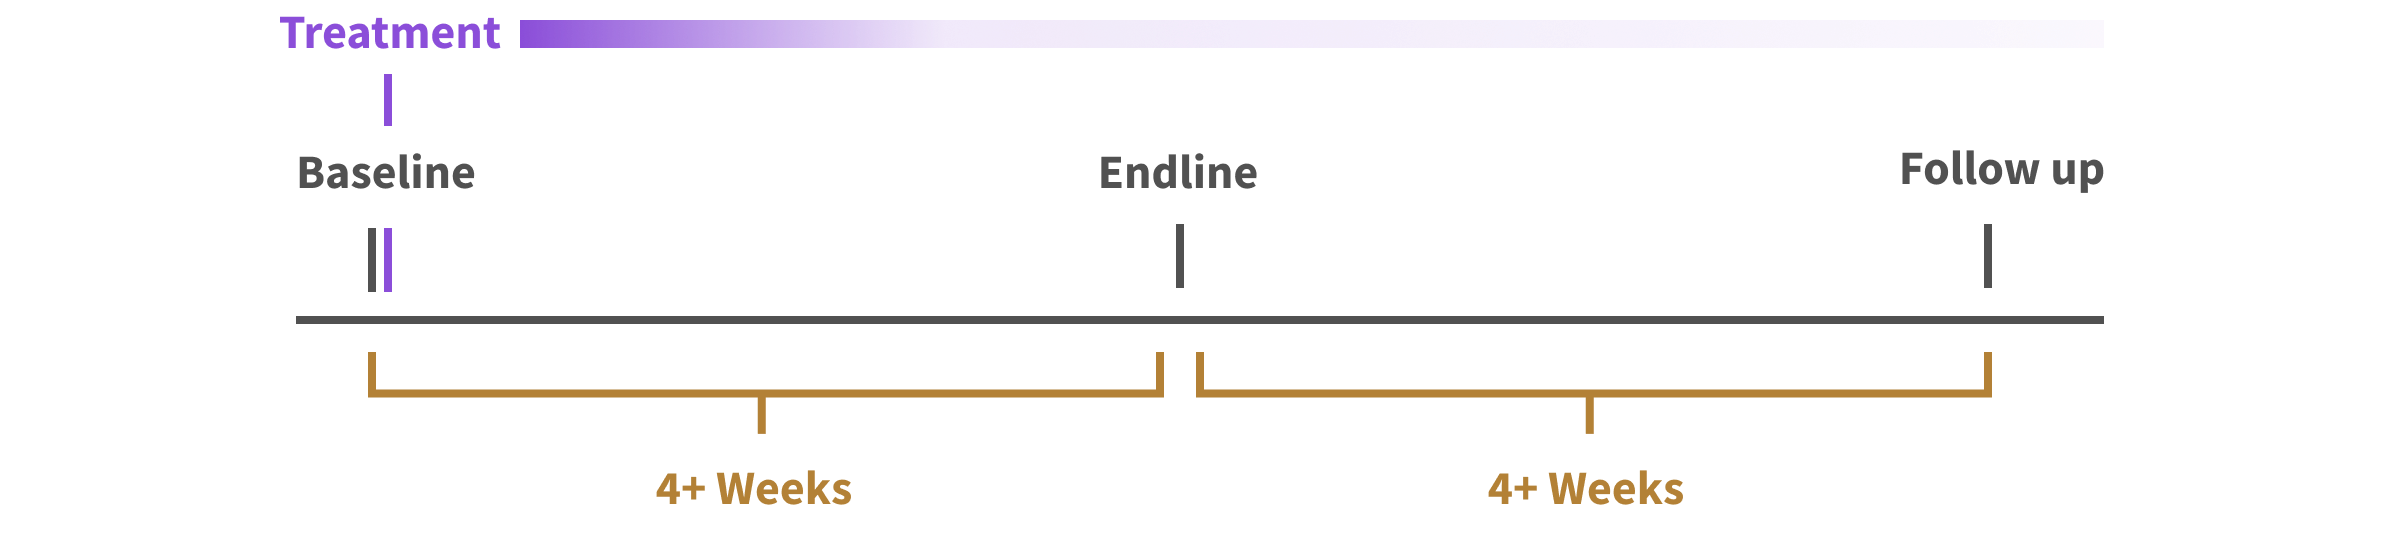
\includegraphics[width=\textwidth]{images/design-timeline.png}
\caption{Study Design}
\label{fig:Study Design}
\end{figure}
\end{frame}


\begin{frame}
\frametitle{Findings}

The analysis conducted on the effects of promoting the Bebbo app on caregivers with children aged 0-6 did not reveal any statistically significant impact on key outcomes of interest. 

One of the main contributing factors to this outcome appears to be the low engagement levels of users with the app. For an app to influence behaviors and attitudes, it must be attractive and engaging enough to retain a large portion of the target audience over time. 



\end{frame}

\begin{frame}
   \frametitle{Findings}

Data indicate that a significant proportion of users tend to abandon the app after a short period. Specifically, 76\% of users in our study who complied with the suggestion to download Bebbo abandoned it after the first day. This is in line with app usage data outside of our study, which shows that over 80\% of users abandon it after one day. 

We additionally find that only 3\% of respondents used Bebbo more than 3 times in a 30 day period. Bebbo’s theory of change is anchored in regular app usage by parents – the current usage rate is unlikely to lead to impact change.

\end{frame}

\begin{frame}
   \frametitle{Findings}
  Additional findings that might have contributed to the lack of measured significant impact included: 

  \begin{enumerate}
  \item There seemed to be a priming effect of the baseline survey, especially for questions related to knowledge, such as “when is your child’s next vaccination due.” This could imply that a prompt itself can change parent’s knowledge and raises questions on how best to position Bebbo in regards to this outcome. 
  \item The majority of respondents scored well on the baseline assessment. If the respondents were representative of the general population, this would imply that most caregivers in these countries are already knowledgeable and following many good practices.
  \end{enumerate}
    
\end{frame}

\begin{frame}
   \frametitle{Recommendations}

\textbf{Improve app targeting}

The 5\% of downloaders that remain as regular users, as well as other suggestive evidence, indicate that Bebbo may work for specific sub-groups. These groups need to be better understood to improve app outreach and uptake strategies. It might be that new implementation modalities would be required to reach these groups. The current shift towards implementing through services providers (i.e., a hybrid strategy) might provide a solution, but it needs to be tested before being scaled up.  

\end{frame}

\begin{frame}
   \frametitle{Recommendations}

\textbf{Adjust app focus based on context}

Considering the high baseline scores of participants, it might be valuable (in places with already better than average parenting knowledge) to consider a focus on particular practices (i.e. breastfeeding) that are still lagging, or groups which are lagging in all practices. 
\end{frame}

\begin{frame}
   \frametitle{Recommendations}
 

\textbf{Adjust app focus based on the comparative advantage to generate knowledge}

The findings suggest that  for many of the targeted outcomes, awareness itself is an effective intervention. This suggests that some outcomes (such as vaccine knowledge) might be more effective through other media and an app should focus on the outcomes that require sustained engagement. 
\end{frame}

\begin{frame}
     \frametitle{Recommendations}
\textbf{Improve app usage}

The current retention and usage rates are not sufficient for Bebbo to have any meaningful impact. Steps should be take to make the app more engaging for caregivers (and service providers considering the new implementation modality). These implementation issues should be addressed through formative and quantitative research  (e.g., User experience (UX) studies to understand what would drive better user engagement, acceptability, accessibility, and reach) before further scaling the app.  

\end{frame}

\begin{frame}
\frametitle{Recommendations}       

\textbf{Adopt an agile approach to evidence generation}

As Bebbo continues to scale, it will need to adopt a more rigorous and agile approach for evidence as well. The team can borrow methodologies from the private sector and use A/B testing, longitudinal analysis of users, and other evaluative approaches to guide decisions around product improvement and iteration2.  This shift towards an agile product development cycle, aligning the evidence generation and innovation cycles, would let Bebbo scale up in a more informed way.  
\end{frame}

\begin{frame}
   \frametitle{Findings and Recommendations}

  In conclusion, while the promotion of the Bebbo app did not result in significant effects on the target population, the study provides valuable insights into the challenges of promoting and sustaining engagement with mobile apps for parenting. 

Future interventions should consider strategies to enhance user engagement and retention to maximize the potential impact of mobile apps in promoting positive parenting practices and knowledge. 
\end{frame}


\message{ !name(bebbo-presentation.tex) !offset(6) }

\end{document}

%------------------------------------------------